Analiza la figura geométrica obten la expresión algebraica para el \textbf{perímetro} de las siguientes figuras:

\begin{table}[H]
    \rowcolors{1}{}{lightgray!20}
    \centering
    \caption{Áreas}
    \label{tab:3.13}
    \begin{tabular}{|c|p{4cm}|c|p{4cm}|}
        \toprule                 \rowcolor{colorrds!80}
        \textbf{\color{white}Figura}                                     & \textbf{\color{white}Área}      & \textbf{\color{white}Figura}                                     & \textbf{\color{white}Área}    \\ \midrule
        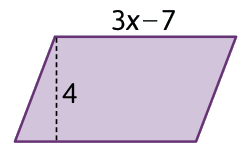
\includegraphics[width=0.2\linewidth]{../images/20230319042726}  & \ifprintanswers $A=4(3x-7)$ \fi & 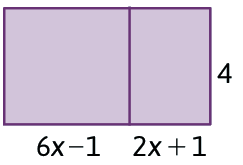
\includegraphics[width=0.13\linewidth]{../images/20230319042743} & \ifprintanswers $A=32x$ \fi   \\ \hline
        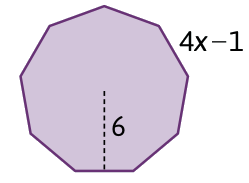
\includegraphics[width=0.14\linewidth]{../images/20230319042734} & \ifprintanswers $A=108x-27$ \fi & 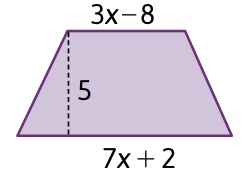
\includegraphics[width=0.18\linewidth]{../images/20230319042750} & \ifprintanswers$A=25x-15$ \fi \\ \hline
        \bottomrule
    \end{tabular}
\end{table}



